\chapter{Desenvolvimento do projeto}
\label{chap:metod}
Nesta seção será descrito o procedimento utilizado para construção de cada um dos desafios.

\section{Webots}
O robô utilizado foi o Pionner o qual usa seus 16 sensores de distância pré-instalados para obter informações do mundo em todas as direções 
e um sensor adcional:o sensor de luminosidade que rastreia a irradiância local e envia um sinal para o robô quando ele lê mais de 750 W / m2, 
o que significa que está perto o suficiente da luminária de chão para disparar o STOP.

\subsection{controle}
A navegação do robô pelo mapa é baseada em uma máquina de 4 estados que determina se ele deve se mover para frente,
virar à esquerda, direita ou parar quando atingir seu objetivo final.

Assim, a divisão foi feita em quatro casos, são eles:
\begin{itemize}
    \item FORWARD: Anda para frente e se houver algum obstáculo à frente ele começa a tomar a decisão de virar em qualquer direção para evitá-lo.
    \item ESQUERDA: Vire à esquerda até que a detecção de objetos não seja mais possível;
    \item DIREITA: Vire à direita até que a detecção de objetos não seja mais possível;
    \item STOP: Quando o sensor de luz detecta a quantidade de luminosidade configurada (neste caso 750 W / m2), o robô deve parar.
\end{itemize}
Todos os sensores de distância coletam dados do ambiente que determinam se o robô deve se mover para frente ou para os lados.
\section{Turtlesim}
Para que o desafio seja cumprido é necessário rodar o roscore e o nó para que a janela da turtle apareça na tela.

\begin{figure} [h!]	
    \centering
    \caption{inicializando o ros}
    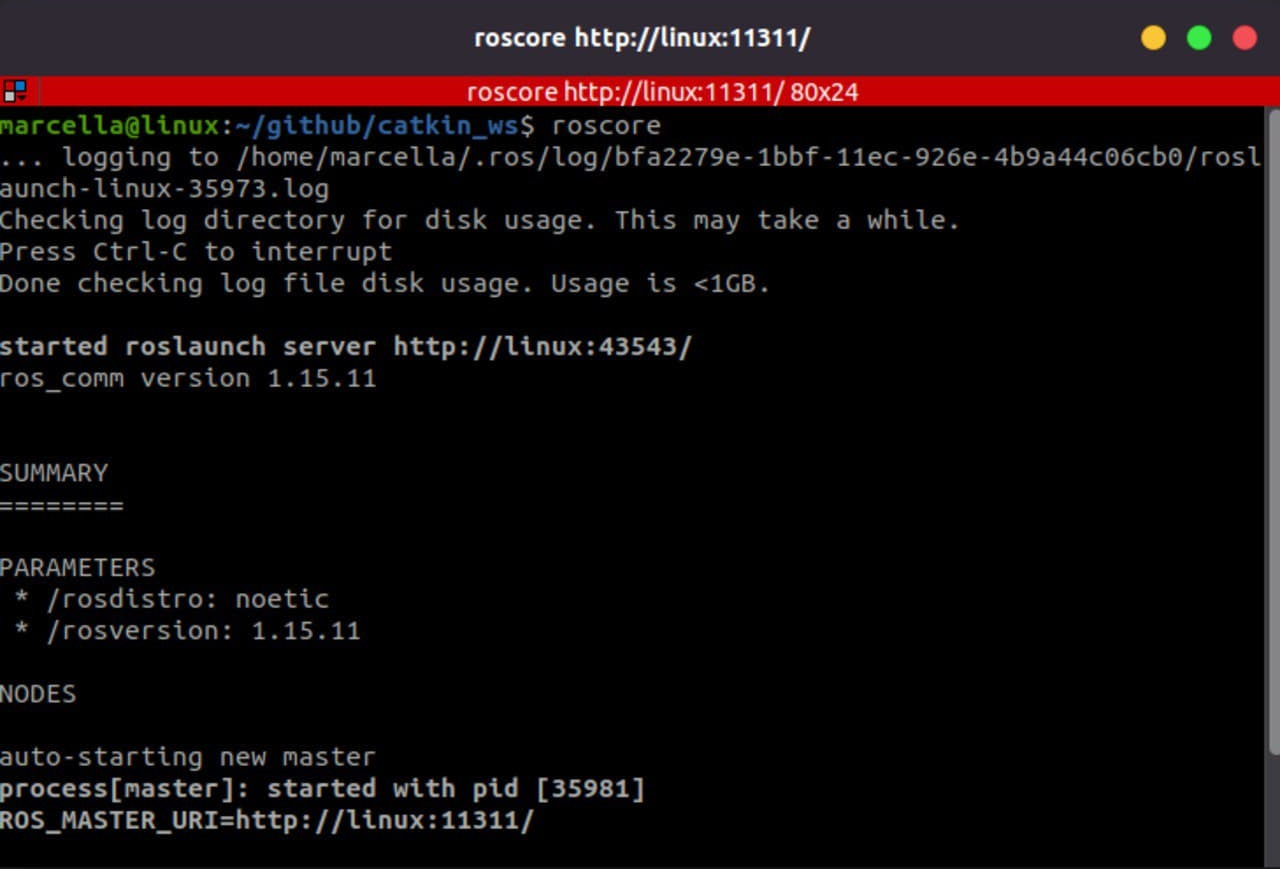
\includegraphics[width=0.5\textwidth]{roscore.jpg}
    \caption*{Fonte: Autoria própria.}
    \label{fig:roscore}
\end{figure}

\begin{figure} [h!]	
    \centering
    \caption{ Rodando o nó do turtlesim}
    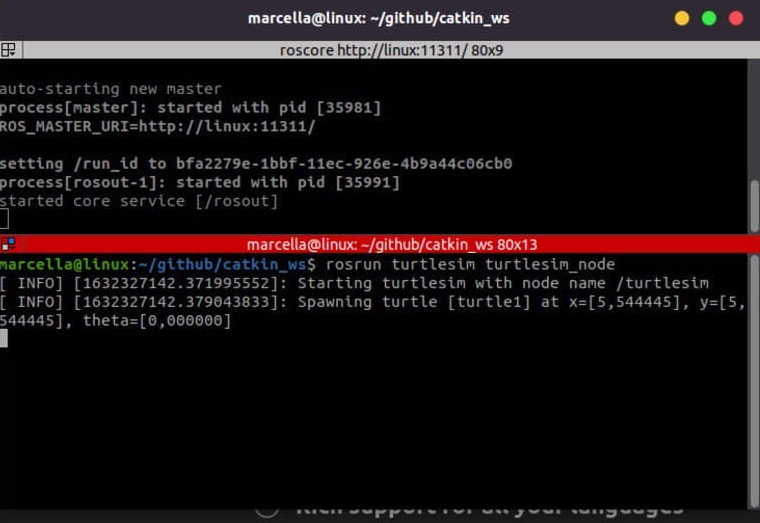
\includegraphics[width=0.5\textwidth]{rosrum.jpg}
    \caption*{Fonte: Autoria própria.}
    \label{fig:rosrum}
\end{figure}
por fim executa-se o arquivo .py quue foi a liguagem escolhida para completar este desafio, como mostra a figura abaixo.
\begin{figure} [h!]	
    \centering
    \caption{ Executando arquivo}
    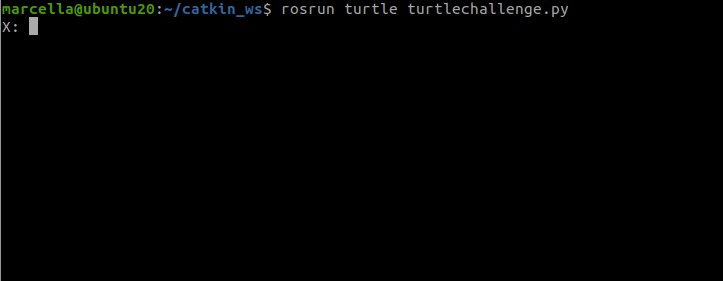
\includegraphics[width=0.5\textwidth]{xey.jpeg}
    \caption*{Fonte: Autoria própria.}
    \label{fig:excute.py}
\end{figure}
É posto as coordenadas x e y no caso do exemplo do desafio é 1 e 1 e a tartaruga deve ir até essa coordenada quando o erro for no máximo 0.1.
\section{Husky}
\textit{Quality Function Deployment} é uma ferramenta de qualidade que auxilia na conversão das demandas do cliente em características de qualidade do produto. Dessa forma, no primeiro ciclo do QFD foram analisados os requisistos do cliente e os requisitos técnicos necessários, sinalizando os pontos mais importantes e as relações entre estes. O resultado foi exposto na \ref{fig:QFD}

\begin{figure} [h!]	
    \centering
    \caption{ Primeiro ciclo QFD}
    \includegraphics[width=0.8\textwidth]{Figures/QFD}
    \caption*{Fonte: Autoria própria.}
    \label{fig:QFD}
\end{figure}
 Através do QFD foi possível observar 

% %--------- NEW SECTION ----------------------
% \section{Interface do Usuário}
% \label{sec:ui}
% \lipsum[1]

% %--------- NEW SECTION ----------------------
% \section{Simulação do sistema}
% \label{sec:sim}
% \lipsum[2-4]

